%=============================================================================
% Thesis Template in LaTex
%
% File:  06-Diskussion.tex -- Diskussion
% Author(s): Cyrano Golliez <golliezc@student.ethz.ch>
%
% Creation:  27 Jan 2014
% Time-stamp: <Tue 2013-08-13 20:14 juergen>
%
% Copyright (c) 2014 Infrastructure Management Group (IMG)
%               http://ibi.ethz.ch
%
% More information on LaTeX: http://www.latex-project.org/
%=============================================================================

\chapter{Diskussion}
\label{chap:Diskussion}

In diesem Kapitel wird die in Abschnitt \ref{chap:Resultate} als optimal erachtete Lösung untersucht. Einerseits werden die Zustände 1 bis 4 mit dem Grundzustand 0 verglichen und andererseits die einzelne Kostenstrukturen in den verschiedenen Zuständen untersucht. Dies geschieht, um die als optimal erachtete Variante auf ihre Belastbarkeit in einer allfälligen Diskussion zuprüfen.

\paragraph{Zustand 0}

Gemäss dem Risikovergleich in Abschnitt \ref{chap:Resultate} ist im Zustand 0 die bestmögliche Variante für die Zukunft von Uster die Variante 2.  
Bei näherer Betrachtung der in Abbildung \ref{img:KostenZ0} dargestellten Reisezeitkosten und Unterhaltskosten der Varianten wird verdeutlicht, dass die Kosten die in der Variante 1 aufgrund der verlängerten Wartezeit entstehen, die Mehrkosten infolge Bau und Wartung der Variante 2, bei einer Betrachtung der Gesamtkosten über einen Zeitraum von 40 Jahren, um ein vielfaches übersteigen. Die Mehrkosten die bei der Ausführung der Variante 2 infolge höherer Bau- und Wartungskosten enstehen, betragen 1'238'600 CHF wohingegen die Mehrkosten die infolge der Variante 1, aufgrund der höheren Reisezeitkosten entstehen 38'984'439 CHF betragen. 

Durch diesen Vergleich wird verdeutlicht, dass sich die Variante 1, welche die Option "nichts zu verändern" darstellt, über den betrachteten Zeitraum von 40 Jahren nicht lohnenen wird. Die Mehrkosten die den Nutzern des Bahnübergangs und somit auch indirekt der Stadt Uster infolge der verlängerten Wartezeit entstehen, übersteigen die geforderten Inverstitionskosten für den Bau der Velounterführung um ein vielfaches. Im Fall der Variante 3 trifft dies nicht zu, weshalb sich ein solches Inverstment unter den Annahmen des Grundzustandes nicht lohnt.

\begin{figure}[h!]
  \centering
  \subfloat[][]{\label{img:}\includegraphics[width=.45\textwidth]{./figures/06-01-Unterhaltskosten-Z0}}
  \hfill
  \subfloat[][]{\label{img:}\includegraphics[width=.45\textwidth]{./figures/06-02-Reisezeitkosten-Z0}}
\caption[Verkehrsaufkommen]{Tägliches Verkehraufkommen Brunnenstrasse}
  \label{img:KostenZ0}
\end{figure}

\begin{IMleftrightskip}
Die Kosten wurden analog der in Abschnitt \ref{subsec:BerechnungRisiken} erläuterten Risikoberechnung ermittelt. Dies gilt für alle weiteren erwähnten Kostenstrukturen.
\end{IMleftrightskip}

Demnach lohnt sich der Bau der Variante 2 für die Stadt Uster bei einer Betrachtung der Gesamtkosten über 40 Jahre und das entstehende Risiko rechtfertigt die höheren Investitionskosten zu Beginn des untersuchten Zeitraum. 

\paragraph{Zustand 1}

Gemäss Abschnitt \ref{chap:Resultate} ist auch in Zustand 1 die Variante 2 die optimale Lösung. Somit hat die Veränderung des E-Auto Anteiles keinen Einfluss auf die Wahl der optimalen Variante. \\
Infolge des Vergleichs der Zustände 0 und 1 ist ersichtlich, dass das Risiko der Variante 1 um 0.023\%, das Risiko der Varianten 2 um 0.024\% und das Risiko der Variante 3 um 0.017\% gegenüber dem jeweiligen Risiko im Zustand 0 ansteigt. Diese Abweichungen wäre, um den Effekt der die Veränderung des E-Auto Anteiles auf optimale Lösung hat, im Rahmen einer Hauptstudie zu untersuchen.

Bei der näheren Betrachtung der Umweltkosten wird ersichtlich, dass die Umweltkosten für alle 3 Varianten jeweils um einen Betrag von 163'555 CHF ansteigen. 
Ein konservative Prognose des E-Auto Anteil hat somit keinen Einfluss auf die Wahl der optimalen Variante. Demnach müsste die Variante 2 auch in einer Zukunft in der der Verbrennungsmotor weiterhin eine massgebende Rolle spielen wird, die als optimal zu erachtetende Variante sein, um die Verkehrssituation am Bahnübergang nachhaltig zu verbessern.


\paragraph{Zustand 2} 

Wie im Abschnitt \ref{chap:Resultate} dargestellt, hat die Veränderung der Unfallwahrscheinlichkeit keinen Einfluss auf die Wahl der optimalen Variante. 
Bei näherer Betrachtung der Unfallkosten, sieht man, dass sich die Veränderung der Unfallwahrscheinlichkeit deutlich auf die anfallenden Unfallkosten auswirkt. 
Die Abbildung \ref{img:UnfallVer.Z0-2} zeigt den Unfallkostenvergleich der Zustände 0 und 2. Die Unfallkosten aller Varianten im Zustand 0 betragen 451'469 CHF. Im Zustand 2 betragen die Unfallkosten der Variante 2 547'384 CHF und die Unfallkosten der Variante 3 321'649 CHF. Für die Variante 2 entspricht das einer Veränderung von 21.25\% und für die Variante 3 einer Abnahme von 28.75\%. 

\begin{figure}[h!]
	\centering
	\includegraphics[width=.45\textwidth]{figures/06-03-Unfallkostenvergleich-Z0-Z2}
	\caption[Unfallkostenvergleich: Zustand 0 und 2]{Unfallkostenvergleich: Zustand 0 und 2}
	\label{img:UnfallVer.Z0-2}
\end{figure}

Betrachtet nun hingegen die Veränderung der Risiken der Variante von Zustand 0 zu Zustand 2, so beträgt die Veränderung für die Variante 1 +0.01\% und für die Variante 3 -0.01\%. 
Somit ist die Variante 2 auch mit erhöhter Unfallgefahr die optimale Variante für die zukünftige Situation am Bahnübergang Brunnenstrasse. 
 

\paragraph{Zustand 3} 

Die Veränderung der Eintrittswahrscheinlichkeit, wie in Abschnitt \ref{subsec:Sensitivitätsanalyse} dargestellt, hat keinen Einfluss auf die Wahl der optimalen Variante. Jedoch ist die folgende Darstellung \ref{img:SzeVer-Z0} der Risiken der einzelnen Szenarien, insofern interessant, dass es den Effekt verdeutlicht der die Wahl der Eintrittswahrscheinlichkeit auf die Verteilung der Risiken hat. So kann mit der Gewichtung der möglichen zukünftigen Ereignisse, sprich den Prognosen der möglichen Zukunft, die berechneten Risiken beeinflusst werden. 

\begin{figure}[h!]
	\centering
	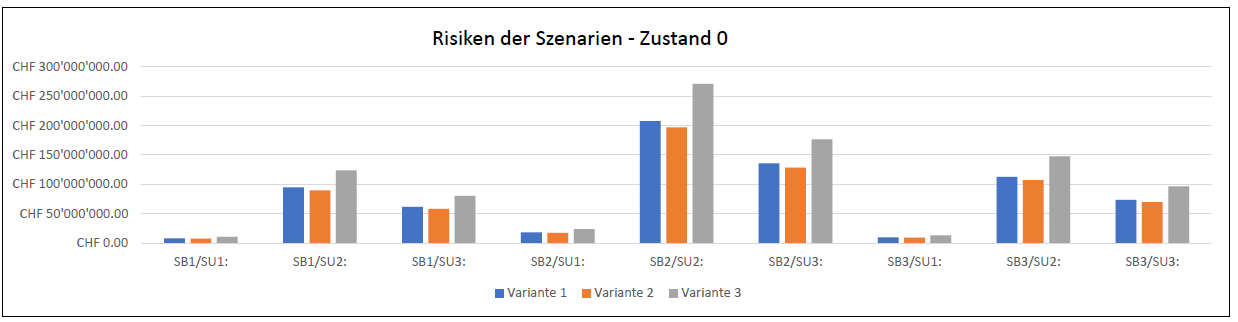
\includegraphics[width=.45\textwidth]{figures/f-06-04-RisikenSzenarienZ0}
	\caption[Szenarienvergleich im Zustand 0]{Vergleich der Risiken der Szenarien im Zustand 0}
	\label{img:SzeVer-Z0}
\end{figure} 

Im Zustand 3 wird der Schwerpunkt der Gewichtung der Szenarien so gelegt, dass diejenigen Szenarien mehr gewicht erhalten, welche die höchsten Wachstumsprognosen voraussagen und demnach das grösste Verkehrsaufkommen simulieren. Der Effekt einer solchen Verschiebung auf die Szenarien wird in der nachfolgenden Abbildung \ref{img:SzeVer-Z3} verdeutlicht. 

\begin{figure}[h!]
	\centering
	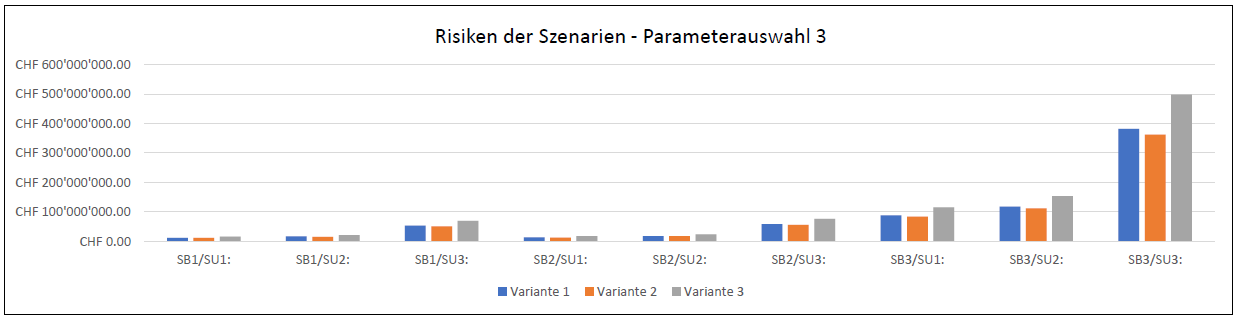
\includegraphics[width=.45\textwidth]{figures/f-06-05-RisikenSzenarienZ3}
	\caption[Szenarienvergleich im Zustand 3]{Vergleich der Risiken der Szenarien im Zustand 3}
	\label{img:SzeVer-Z3}
\end{figure} 

Auf die Wahl der optimalen Variante hat diese Veränderung keinen Einfluss, da die Risiken der Varianten jeweils um 5.5\% im Vergleich zum Zustand 0 steigen. Erst bei der Betrachtung der Nachkommastellen, lässt sich eine gewisse Unterscheidung feststellen. So beträgt die Veränderung des Risiko der Variante 1 vom Zustand 0 zum Zustand 3 5.530\%, die Veränderung des Risiko der Variante 2 beträgt 5.518\% und die Veränderung des Risikos der Variante 3 5.525\%. Aus diesen geringfügigen Abweichung einen Rückschluss auf die im Rahmen des Zustand 3 veränderten Eigenschaften der Risikoberechnung zu machen, war im Rahmen dieser Projektarbeit nicht möglich und wäre im Rahmen einer Hauptstudie weiter zu untersuchen.


\paragraph{Zustand 4} 

in die anderere Richtung die Argumentation gegen die V2 -> fals für alle 3 die wartezeit steigt, weil noch mehr züge kommen, so dass amepelsystem nicht zu extra wartzeit führt, dann aber nur dann wäre die Variante 3 der Variante 2 überlegen... um wie viel...

%Die Kapazität für den ÖV ist in keiner Variante beeinträchtigt. Einen Ausbau der Kapazität ist nicht geplannt. Neubauten oder umstrukturierungen verschiedener Bushaltestellen ist im Rahmen der genaueren Bauausführung zu prüfen. \\

%Hier werden die Resultate diskutiert. 

%Der geplanten Stadterschliessungen West und Süd-Ost sind für die Förderung des Langsamverkehrs in der Stadt Uster von zentraler Bedeutung. So kann eine Entlastung des Zentrums und der Nord-Süd Achse entlang der Bahnhofstrasse nur realisiert werden wenn der MIV entlang der Westumfahrung um das Stadtzentrum herum geführt wird. 

%Dies ermöglicht gemäss STEK eine komfortable, durchgehende und direkte Verindung mit allenfals zu prüfender Vortrittsberechtigung. Die Infrastruktur dieser Radwege sollte ausschliesslich für diese Art von Verkehr zugelassen sein und gemäss STEK Kap.7 Tab. 1 mind. 4.8m breit sein. Um eine kreuzungsfreie Durchfahrt zu gewährleisten ist eine Ausführung in Anlehnung an den Aufbau einer Autobahn zu prüfen.  

% ===========================================================================
% EOF
%

%%% Local Variables:
%%% mode: latex
%%% TeX-master: "../main"
%%% End:
